\documentclass[10pt, letterpaper]{article}
\usepackage[top=80pt,bottom=80pt,left=60pt,right=60pt]{geometry}
\usepackage{tabularx}
\usepackage{float}
\usepackage{titling}
\newcommand{\subtitle}[1]{%
  \posttitle{%
    \par\end{center}
    \begin{center}\large#1\end{center}
    \vskip0.5em}%
}
\usepackage{pgfplotstable}
\usepackage{tikz}
\usepackage[section]{placeins}
\usepackage[utf8]{inputenc}
\usepackage{csvsimple}

%\pgfplotsset{compat=1.11}

\begin{document}

\title{Internal Assessment: The Impact of the Sphere's Radius on the Sphere's Angular Velocity}
\subtitle {IB Physics II Period 6, Dr. Petach}
\date{19 October 2015}
\author{Jackson Chen}
\maketitle

\section{Design}

\subsection{Research}

The aim of the experiment is to investigate the relationship between period and height for the circular motion of an airplane
moving in a circle at equilibrium. This will be done by changing the length of the string that the airplane is attached to and then measuring
the period and the height of the airplane's flight with a stopwatch and a laser, and a meter stick, respectively.

Prior to the experiment, I derived a relationship between the period and the height of the circular motion of an airplane's flight
by using the force analysis of the airplane, the definition of a period, and the radius of the flight path. Section 2.2.3 will more
specifically detail the derivation. The derived relationship predicted that period and height will follow a square root relationship.
The experiment itself was to test if Newtonian physics upheld this square root relationship with tangible experimentation.

\subsection{Variables}
The independent variable is the length of the string that the airplane is attached to. The dependent variables are the
period and height of the circular motion that the airplane makes. The controlled variables include the mass of the airplane,
material of the string, the timer, the laser, and the properties of the surrounding environment.

\subsection{Apparatus}
\begin{itemize}
  \item Hook
  \item Model airplane
  \item String
  \item Stopwatch (on a phone)
  \item Meter stick
  \item Laser
  \item Ring stand with clamp
\end{itemize}

\subsection{Procedure}
\begin{enumerate}
  \item Attach the model airplane to a 100cm string and connect it to a hook attached to the ceiling.
  \item Turn the airplane on, and wait for the motion to reach equilibrium.
  \item Clamp a laser onto a ring stand and make the laser parallel to the surface that the ring stand is on.
  \item Raise or lower the laser (without changing its angle) so its light hits the moving airplane anywhere in its circular orbit.
  \item Measure the height of the airplane with respect to the ceiling by measuring the placement of the laser with respect to the ceiling with a meter stick.
  \item Use the timer to measure the amount of seconds it takes the airplane to complete three revolutions.
  \item Repeat steps 5-6 five times for five different trials.
  \item Repeat the experiment (for one trial) for strings of lengths: 90cm, 80cm, 70cm, and 60cm.
\end{enumerate}

\subsection{Diagram}
\begin{figure}[!htb]
\centering
\includegraphics[scale=0.5]{Lab1_drawing.png}
\caption{Diagram of apparatus setup}
\end{figure}

\section{Data}

\subsection{Data Collection}
\begin{table}[H]
\centering
%\csvautotabular{data/hackeysack.csv}
\pgfplotstabletypeset[
    col sep=comma,
    string type,
    every head row/.style={
        before row={\hline},
        after row=\hline
    },
    every last row/.style={after row=\hline},
    ]{data/hackeysack.csv}
\caption{Data for a string length of $100 \pm 2$cm. The purpose of five trials was to determine uncertainty.}
\end{table}

\begin{table}[htp]
\begin{tabularx}{\linewidth}{>{\centering\arraybackslash}X>{\centering\arraybackslash}X>{\centering\arraybackslash}X }
\hline \textbf{String length (cm)} & \textbf{Height (cm)} & \textbf{Time per 3 revs(s)} \\ \hline
$90 \pm 2$ & 57.95 & 4.58 \\ \hline
$80 \pm 2$ & 46.85 & 4.51 \\ \hline
$70 \pm 2$ & 37.92 & 3.95 \\ \hline
$60 \pm 2$ & 42.24 & 3.85 \\ \hline
\end{tabularx}
\caption{Data for four different string lengths}
\end{table}

\subsection{Data Processing}
\subsubsection{Averaging the five trials for a string length of $100 \pm 2$cm}
The average heights over the five trials for a string length of $100 \pm 2$cm is:
\[ \frac{71.30 + 70.11 + 69.45 + 67.50 + 66.98}{5} = 69 \pm 2cm \]
The uncertainty is calculated by dividing the range by 2. The average time per 3 revolutions over the five trials for a
string length of $100 \pm 2$cm is calculated in the same way:
\[ \frac{4.89 + 4.90 + 5.03 + 5.03 + 5.01}{5} = 4.97 \pm 0.07s \]
The uncertainties that were just calculated will be applied to the rest of the data, as the purpose of performing five trials
was to determine the uncertainty for height and time per 3 revolutions.
\subsubsection{Calculating Period}
The period of the plane's circular flight, is the seconds per 1 revolution. Since the time per 3 revolutions is a measured quantity,
the period can be calculated by dividing that value by 3. For example, the period for string length $100 \pm 2$cm is:
\[ \frac{4.97 \pm 0.07}{3} = 1.66 \pm 0.07s \]

After processing the data in sections 2.2.1 and 2.2.2, Tables 1 and 2 can be consolidated into one table, as well as have
uncertainty appended to the height and time per 3 revolutions columns. A new column for period can be added as well. This will be presented in Table 3.

\begin{table}[H]
\begin{tabularx}{\linewidth}{>{\centering\arraybackslash}X>{\centering\arraybackslash}X>{\centering\arraybackslash}X>{\centering\arraybackslash}X }
\hline \textbf{String length (cm)} & \textbf{Height (cm)} & \textbf{Time per 3 revs(s)} & \textbf{Period (s)} \\ \hline
$100 \pm 2$ & $69 \pm 2$ & $4.97 \pm 0.07$ & $1.66 \pm 0.07$ \\ \hline
$90 \pm 2$ & $58 \pm 2$ & $4.58 \pm 0.07$ & $1.53 \pm 0.07$ \\ \hline
$80 \pm 2$ & $47 \pm 2$ & $4.51 \pm 0.07$ & $1.50 \pm 0.07$ \\ \hline
$70 \pm 2$ & $38 \pm 2$ & $3.95 \pm 0.07$ & $1.32 \pm 0.07$ \\ \hline
$60 \pm 2$ & $42 \pm 2$ & $3.85 \pm 0.07$ & $1.28 \pm 0.07$ \\ \hline
\end{tabularx}
\caption{Consolidated table with 5 string lengths, period, and uncertainty}
\end{table}

\subsubsection{Deriving a relationship between period and height}

\begin{figure}[!htb]
\centering
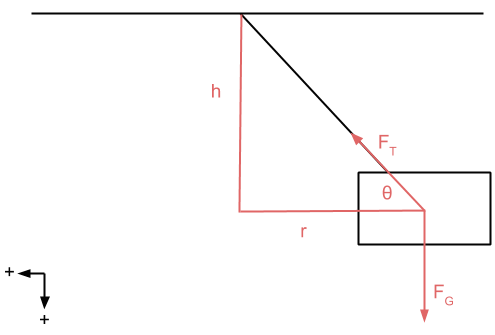
\includegraphics[scale=0.5]{Lab1_FreeBody.png}
\caption{Free Body Diagram of Airplane}
\end{figure}


As mentioned in Section 1.1, the purpose of the investigation was to test if experimental data supported a derived relationship between
period and height. This derivation is as follows:

\[\Sigma F_{y} = 0 = F_{G} - F_{Ty} = mg - F_{T}*\sin \theta \]
\begin{equation}
F_{T} = \frac{mg}{\sin \theta}
\end{equation}
\[\Sigma F_{x} = ma = F_{Tx} = F_{T}\cos \theta = F_{c} = \frac{mv^2}{r} \]
By the definition of period, $T = \frac{2\pi r}{v}$. Therefore $v = \frac{2\pi r}{T}$, which can be substituted in:
\[F_{T}\cos \theta = \frac{m}{r} * \left(\frac{2\pi r}{T}\right)^2 \]
From Figure 2, we can see $r = \frac{h}{\tan \theta}$. Substituting r, and $F_{T}$ from Equation 1:
\[mg\frac{\cos \theta}{\sin \theta} = \frac{m}{\frac{h}{\tan \theta}}*\left(\frac{2\pi h}{T\tan \theta}\right)^2 \]
\[mg\cot \theta = \frac{m\tan \theta}{h}*\frac{4\pi ^2 h^2}{T^{2}\tan ^2 \theta} \]
\[g\cot \theta = \frac{4\pi ^{2}h}{T^{2}\tan \theta}  \]
\[T^2 = \frac{4\pi ^{2}h}{g}  \]
\begin{equation}
T = 2\pi \sqrt{\frac{h}{g}}
\end{equation}

\begin{figure}[H]
\centering
\begin{tikzpicture}
\begin{axis}[
  legend pos=outer north east,
  title={Period vs Square Root of Height for a Circulating Plane at Equilibrium},
  xlabel={Square Root of Height ($\sqrt{cm}$)},
  ylabel={Measured Period (s)},
  xmin = 6,
  xmax = 8.5,
  ymax = 1.8,
  ymin = 1.1,
  scale = 1.5
]
\addplot[scatter, only marks,
        error bars/.cd,
            y dir=both,
            y explicit,
            x dir=both,
            x explicit,
    ] table[x=X,y=Y,y error=Y_error, x error = X_error] {data.dat};
\addplot [thick, red] table[
    y={create col/linear regression={y=Y}}
] % compute a linear regression from the input table
{data.dat};
\addplot [blue, no markers] coordinates {(6.6,1.21) (8.2,1.73)};
\addplot [green, no markers] coordinates {(6.4,1.35) (8.4,1.59)};
\addlegendentry{Data}
\addlegendentry{%
$ y = \pgfmathprintnumber{\pgfplotstableregressiona} \cdot x
        \pgfmathprintnumber[print sign]{\pgfplotstableregressionb}$}}
\addlegendentry{$y =  0.33 \cdot x - 0.94$}
\addlegendentry{$y = 0.12 \cdot x+ 0.58$}
\end{axis}
\end{tikzpicture}
\caption{Graph of T vs $\sqrt{h}$ with line of best fit, maximum slope, and minimum sloped lines.}
\end{figure}

The maximum gradient is 0.33 and the minimum gradient is 0.12. The best fit line gradient is 0.17. \\
The uncertainty above the best fit line is $0.33 - 0.17 = 0.16$ \\
The uncertainty below the best fit line is $0.17 - 0.12 = -0.05$ \\
The gradient, including uncertainty is $0.17 \cdot \frac{0.16}{-0.05} = \boxed{0.17 \pm 0.11}$

\section{Conclusion}
The gradient means that $\sqrt{h}$ increases with T by a proportionality factor of 0.17 $\frac{\sqrt{cm}}{s}$
with an uncertainty of \pm 0.11.

According to Equation 2, the slope that was predicted by the derived relationship is:
\[ \frac{T}{\sqrt{h}} = \frac{2\pi }{\sqrt{g}} = 2.0 \frac{\sqrt{m}}{s} = 0.2 \frac{\sqrt{cm}}{s} \]

We can perform a percent error analysis on the slope:

\[ \frac{|0.2 - 0.17 \pm 0.11|}{0.2} \cdot 100 = 15 \pm 10 \% \]

\subsubsection{Evaluation}
The relationship between T and $\sqrt{h}$ is relatively justified with the data, due to its small percent error compared with the calculated slope.
However, errors involved were rather significant since the gradient varies by 65\% ,which is high. A potential source of error includes the changing of
the laser in the middle of the experiment, due to the battery running out in our laser in the middle of the experiment. The new laser had a much larger
beam of light (in terms of area), and thus measuring the height of the laser dot to the roof was incredibly difficult. Furthermore, the laser dot was
extremely bright and made it difficult to accurately make out the increments in the meter stick. Another source of error came from the timing of the
three revolutions that the model airplane made. The hand-eye coordination let to a delay between noticing when the laser hit the airplane and hitting
the stop button on the stopwatch. Thus the time measurement for 3 revolutions varied in every trial. Finally, a third source of error could have resulted
from the laser not being perfectly parallel to the table that the ring stand was on.

\subsubsection{Improvements}
There are many improvements that could be made to this experiment to fix many of the sources of error mentioned in Section 3.0.4. For example, instead of
relying on hand-eye coordination to measure the time it takes for the airplane to make three revolutions, there could be a machine on the other side of the
laser beam that detects if the light beam has been cut off (i.e when the airplane has flown in front of the laser beam). Once that is detected, the stop time
would become extremely coordinated. Secondly, placing a gyroscope reader on the laser would allow us to detect how parallel it was relative to the surface.
Finally, a better way to have measured the height was to measure the height directly from the laser to the ceiling rather than from the laser beam (which is
extremely bright).

\end{document}
